\section{Brain visual pathways}
\label{sec:sectionb}

\subsection{The eye}

Most of the visual relevant information we receive consists of spatial and time variations in light intensity \cite{Green}. When receiving light, the retina maps the light's temporal and spatial patterns onto a layer of receptor cells that respond to light with an electrical activity pattern in a retinotopical map: organized, topographically ordered representations of the visual field (for textbook reviews, \cite{Purves}, \cite{Kandel}).  

The retina is the innermost layer of the eye, and a part of the central nervous system. It contains light-sensitive neurons, photoreceptors, and allows for the transmission of visual signals through another class of neurons, the ganglion cells. It also contains horizontal, bipolar and amacrine cells. Horizontal and amacrine cells mediate lateral interactions. The major route of information in the retina follows from the photoreceptors to the bipolar cells and finally to the ganglion cells. Each ganglion cell responds by changing its firing rate to stimulation of a roughly circular concentric patch of the retina, its classical \textit{receptive field} \cite{Kuffler1953}. This information is then relayed to the brain.

The photoreceptors, rods and cons, are the first recepients, and account respectively for the sensitivity and the acuity in the detection of light \cite{Green}.
When light falls in the retina's photoreceptors, they are activated by means of graded changes in membrane potentials that then induce corresponding changes in the rate of synaptic transmitter release from ganglion cells. 

To allow the eye to respond efficiently over great spatial and temporal ranges in illumination intensity, this regulation's criteria is based on judicious input's pattern transformations. Both the temporal and spatial conversions code information by means of giving prominence to rapid \textit{changes} and filtering out slow changes in light intensity over time and space.

The temporal frequency in the photoreceptors undergoes \textit{adaptation} - with major impulse rate signals corresponding to a sudden peak in light intensity that is rapidly set back to a lower steady level. The ganglion cell's response rates depend as well on the background level of illumination, with adaptive range shifts that scale the response to a visual scene's illumination levels. In this way, the retina normalizes the received inputs in relation to the full image's statistics. 

Concerning the spatial pattern, the question becomes, how are the different receptors responses jointly treated? In fact, \textit{lateral inhibition} arises: If, while in the dark, a small light stimulus appears, rod cell's will be enhanced. The rod cells corresponding to the center of the stimulus' location will send an activated signal. However, due to lateral inhibition from horizontal cells, the different rod cells outside the stimulus' location will send an inhibitory signal. This implies the prominence of boundaries between bright and dimmed regions.

Both the temporal and spatial transformations code information by means of giving prominence to rapid \textit{changes} and filtering out slow changes in light intensity over time and space. 

The sensitivity to light-dark borders in the visual scene is further achieved by the two ganglion cells classes, on-center and off-center (\cite{Purves}, \cite{Kandel} reviews). These cells are sensitive to differences between illumination levels in its receptive field center and in its ring-shaped surround. In an on-center ganglion cell, brightly illuminating a central spot of the receptive field produces a burst of action potentials. In an off-center cell, the response to the same stimulus is a reduced rate of action potentials, and an increase as the illumination is turned off. In the case of dark spots, the on- and off-center cells show the opposite activity pattern. In this way, there are two separate channels of luminance \textit{changes} being carried to the brain, and either increases or decreases in brightness are always encoded as increased action potentials in the ganglion cells.


%Chapter 3 in 'visual perception', Visual pathways in the brain

%Kandel Principles of Neural Science Book

%Purves Neuroscience Book


\subsection{Central Visual Pathways}

Firstly, the primary visual pathway mediates vision and visual perception. Information is driven from the retina, to the thalamic dorsal lateral geniculate nucleus (LGN) and finally to the primary visual cortex (V1) (for a review, \cite{Purves}, \cite{Kandel}, \cite{Bear}).%, all containing different kinds of neurons for encoding various visual properties.

Ganglion cell's axons follow a path over the retina's surface to the optic disk, bundling together in the optic nerve. %This retina's region is insensitive to light and is therefore responsible for the blind spot - a substancial gap in each monocular visual field. 
From here, the ganglionic axons continue to the optic chiasm, past which the axons from both sides form the optic tract. These axons then continue to the brain, mainly projecting in the dorsal lateral geniculate nucleous (LGN) in the thalamus. The LGN is arranged in layers and appears in both brain hemispheres,  receiving information from the left and right semifields of view detected by each of the two retinas. These then radiate to the striate cortex, in the primary visual cortex V1, mostly to layer 4 (out of 6 functionally distinct ones).

The ganglion cells can also project to the pretectum, an area that treats reflex control of the pupils and lens. Other targets comprise the suprachiasm nucleus of the hypothalamus, controlling the visceral night/day cycle functions and the superior colliculus that coordinates head and eye movement. Each of this routes requires different types of visual information, in terms of its resolution, features detail and properties' measurements. 

In both LGN and V1, the retinotopy is mantained.
As with the retina cells, visual neurons can be described in terms of their receptive field: the visual field area to which the neuron evokes a spiking response when a isolated local stimulus of optimal parameters is presented in that region \cite{Hubel1959}.

In accounts for these cells stimulus response organization, the LGN cell's receptive fields are concentric and ruled analogously to those from the ganglion cells. 
However, the striate cortex's V1 cells can have different organizations of their receptive fields, with different distributions and numbers of excitatory and inhibitory areas. 

Furthermore, neurons in the striate cortex have an added property: they can be tuned, and present selectivity to particular features. A neuron's tuning can be specified for any stimuli space, and its responsiveness measured for different points within that space. 

Foremost, the response of neurons in cortical areas such as V1 is found to be tuned to orientation of edges \cite{Hubel1959}. The orientation to which a given cell produces the larger response is called the preferred orientation of the neuron, and all orientations are equally represented in the visual cortex. For cats and primates, V1 neurons are mostly organized in columns of different selectivity to particular stimuli attributes: Across layers, in the same direction, neurons respond to the same orientation. Hence, receptive fields are repeatedly represented into modular sheets of neuron distributions in each sublayer. Furthermore, some cortical neurons are selective to lengths or to the direction of stimuli bars, to color, spatial frequency or ocular preference - relative strength of the input from the two eyes. 

Following from V1, extrastriate cortical areas are organized into two large systems: The ventral stream, following V1 to V2 to V4 and connecting to the temporal lobe, thought to account for object recognition, high-resolution images treatment; and the dorsal stream, with a path from V1 to V2 to MT and connecting to the parietal lobe, thought to process the analysis of motion and positional relations between objects in a visual image, as well as attention control. Accordingly, neurons in the ventral stream are selectively tuned to shape, color, texture and, in higher levels, to faces and objects. It is however important to note that, for example, a given specific face's recognition is encoded by a specific pattern of activity in a population of cells, and not by the unique firing of a super-narrowly specific cell. On the other side, dorsal stream's neurons are selective to elements such as movement's direction and speed, containing a detailed map of the visual field.

Neurons at higher levels in the visual pathway are increasingly tuned, latent, and in general have larger receptive fields.

Ascending away from the striate cortex, an hierarchy can be recognized, evolving from the analysis of simple attributes of an image, such as contrast, colour, orientation of segments, going to intermediate level vision, regarding contour integration and surface segmentation, and finally turning to more complex visual processings such as object recognition. 


\subsection{Feedforward: spatial filtering of natural images}

Ganglion cells can be treated as low-pass spatial filters, producing responses to sinusoidal gratings having different spatial frequencies, with a given range (the neuron's bandwidth) determined by the receptive field's size (\cite{Green}, for an overview). 

The neuron's bandwidth becomes narrower as we go from ganglion to LGN and then to striate cortex cells. 

Particularly, simple cells can, in this sense, be described as Gabor functions \cite{Jones1987}, a product of a sine function and a gaussian envelope. This description accounts for the necessary trade-off in spatial frequency and spatial location specificity: A wider gaussian relates to a wider receptive field and thus a narrower spatial frequency bandwidth, but a larger set of possible stimulating spatial locations. This motivates the idea for the efficient encoding strategy of the natural visual world. In a given image, redundancy is expected: it is probable that the light reaching one photoreceptor will be strongly correlated to the light that reaches its neighbours, and thus, at first levels such as V1, high specificity is not required, and patterns can be more economically encoded.

On the other hand, striate cells can be regarded as bandpass filters, with a greater variation in the allowed spatial frequency tuning. 
The striate cortex processes many differently located patches from the retinal image, each containing different spatial frequencies, with the firing rate of each cell accounting for the amplitude of the frequency component to which the cell is tuned - a patch-wise Fourier analysis of the input image.


\subsection{Feedback pathways and influences}
\label{subsec:feedback}

Up until this point, this description has focused on the classical model of feedforward transmission of sensory information in an hierarchy of cortical visual areas, beginning with V1 and following through the ventral and the dorsal pathways.
However, visual pathways are bidirectional. Superimposed in these bottom-up connections, there are reentrant pathways that transmit influences in the reversed top-down direction, in every stage of the visual pathways except for the retina, from higher order cortical areas to neurons in lower processing levels (\cite{Gilbert2013}, for an overview on feedback effects).

To understand these reciprocal interacting mechanisms that can cause non-linear effects, another point must be made explicit: Neurons do not function as fixed functional processors, but rather as adaptive units that can change their function depending on the behavioral context, subject to attention, expectation and perceptual task instructions, at any given processing moment.

This adaptation appears via both changing of neurons' tunings to stimuli - changing of their receptive fields characteristics - and by alteration of the correlations structure of neuronal ensembles.

The neuron changes its \textit{line label}, in accordance to higher orders instructions: A neuron's response means that a stimulus with its preferred attributes is being detected, being the signal as strong as the stimulus is close to that preferred configuration. However, due to feedback, a cell can function in different functional states and the meaning of the information they convey depends on that state - its preferences are changed. The analysis is not misinterpreted because the higher areas that send the adaptative instruction to a given neuron or population of neurons also process the resulting returning signal.

On the other hand, a network of neurons within the same, as well as across different cortical areas, can change their spatial and temporal distribution of correlated activity. In fact, if neurons can be made independent to one another, an ensemble of such neurons will have less variability than that of a single neuron's response to a given stimulus, allowing for better signal to noise ratios of that process and thus for more optimal information encoding.

Vision is then seen as an active process, with feedback conveying signals that adapt the lower neurons in such a way that allows them to encode more relevant information within a given contextual paradigm, facilitating the visual scene representation and interpretation: Their responses to a stimulus are made more informative about the identity of that stimulus. Moreover, given the complexity of the neural pathways, this idea implies that any given cell receives input, directly or indirectly, through feedforward or feedback entrances, from each other relevant processing stage, in a way representing the full brain on their own.

%Beyond a straightforward low-level analysis of simple local attributes, under feedback influences, neurons can integrate six main different forms of contextual information: Spatial, object and feature oriented attention; the at hand perceptual task; object expectation; another behavioural context effect is the case of eye movement across a visual scene. For the image to continue appearing stable, an efference copy of the motor instruction for the eye movement is kept in higher cortical levels and this information is then sent to the retina that compensates for that signal; Finally, top-down influences can also provide memorized and learned information. 

Beyond a straightforward low-level analysis of simple local attributes, under feedback influences, neurons can integrate six main different forms of contextual information\cite{Gilbert2013} firstly, spatial attention can enhance some responses and suppress others outside the attention focus, facilitating the selection of behaviourly relevant stimuli from distracters. second, the discriminability of features of the same object - object oriented attention - and components with similar characteristics - feature oriented attention - can as well be enhanced. The neurons' tuning can also change according to the perceptual task at hand, allowing for the discarding of irrelevant stimuli information to the considered task. Object expectation can also play a feedback role, when a subject is cued to seek for a specific shape.  Finally, top-down influences can also come as working memory, associative memory and perceptual learning information, with prior experience at shorter and longer term yielding important processing instructions. 

Feedback thus enables neurons to process information from contextual influences, relating to larger parts of the visual field and these can as well become selective to more global visual scene configurations. Moreover, feedback has also been implicated in making each neuron's response more relevant, more informative and sparse in the individual's context.

%Feedback: Some forms of these signals appear as predictive hypothesis testings, as higher-levels predict an image from the lower-level activity, and this is carried back with an error signal between the prediction and the stimulus-based signal.


\section{Surround modulation in the visual cortex}

Thought to underlie optimal coding efficiency, sensory processing, spatial integration and global scene perception, sensory neurons exhibit the surround modulation phenomenon: 


If a stimulus is presented, optimally-oriented, in the RF area of a neuron(\textit{center} ), this neuron will fire a response. If it is presented outside that RF area(\textit{surround}), then no response will take place, by definition. However, if jointly presented in both center of the RF and its surround, a modulation of the neuron's signal will take place. This facilitatory or inhibitory modulation will depend on the relative stimuli characteristics in both locations. 

This property was initially found in cat V1 \cite{Hubel1965}, and has currently been shown to occur in many species - mouse \cite{VanDenBergh2010}, cat \cite{Blakemore1972}, monkey \cite{Cavanaugh2002a}; in humans, spatial context has been shown to alter the perception of a visual target (for example, \cite{Chubb1989}, \cite{Cannon1991}, \cite{Nurminen2009} -, sensorial systems and processing levels, ranging, for the visual system, from the retina \cite{McIlwain1964}, \cite{Solomon2006} to neurons in the extrastriate cortex \cite{Allman1985}. 

It has been particularly studied in the visual system, area V1 (\cite{Hubel1965}, \cite{Blakemore1972}, \cite{Maffei1976}, \cite{Gilbert1977}, \cite{Cavanaugh2002a}, \cite{VanDenBergh2010}; for a review, \cite{Angelucci2017}).

Typically, visual SM is studied with either of two methods: An expanding circular grating patch, or RF grating patches surrounded by gratings in an annulus, whose gratings parameters are made vary sistematically (for a review, \cite{Angelucci2017}).

Summarily, SM in V1 has been described with five main attributes: 

\begin{itemize}
\item First, it is spatially extensive, with SM strength decreasing with distance from the neuron's RF (\cite{Cavanaugh2002a}, \cite{Shushruth2009});

\item Secondly, SM effect's sign and strength are also dependent on the strength of stimuli activation in both the RF and the surround - stimulus size, orientation optimality and contrast levels. In fact, when the RF is strongly stimulated (high contrast, optimal orientation and size stimulus), either weakly (low contrast or suboptimal orientation or size stimulus) or strongly activated surrounds will cause a suppressive effect. Conversely, when the RF is weakly activated, strongly activated surrounds will also evoke suppression, but weakly activated surrounds can lead to facilitatory modulation (\cite{Ichida2007}, \cite{Shushruth2012}).

\item Moreover, SM is fast, and can be described in two temporal components: The earliest is untuned to the stimulus properties and can occur at the onset of the RF response with no delay \cite{Henry2013}, nearly independently from the distance of the surround stimulus \cite{Bair2003}. The later component is tuned and $10-30 ms$ delayed in relation to the onset of RF responses \cite{Bair2003}.

\item Additionally, SM properties are different across cortical layers: In layer 4C that does not receive feedback relay, but inputs from the LGN, SM is weaker, untuned for orientation and less spatially expansive than for any other layer. On the other hand, for more superficial layers 4B and above, SM is stronger and more sharply tuned for orientation than for the deeper layers.

\item Finally and most importantly, SM is tuned to specific stimulus parameters, suppressing more strongly responses for stimuli in the RF and surround with the same orientation, spatial frequency, drift direction and speed and either weekly suppressing or even enhancing the signals for orthogonal parameters ( \cite{Cavanaugh2002a}, \cite{Henry2013}, \cite{Self2014}). This differentiated effect appears even if the RF stimulus is not at the neuron's preferred orientation: the stronger suppression for iso-oriented stimuli is present provided that the RF stimulus evokes a response when presented alone, even if this is not the maximal response.

\end{itemize}
SM has been implicated with a variety of possible visual processes and functions.

From its property of evoking stronger responses for dissimilar stimuli inside and outside a neuron's RF, SM can evoke visual saliency, perception of object boundaries, and figure-ground segregation (\cite{Nothdurft2000},\cite{Lamme1995}), by enhancing neuronal responses in discontinuity areas.

Secondly, another reported SM effect is that small collinearly aligned line segments with the same orientation can lead to facilitated responses. This suggests a SM function for contour integration, aiding in the detection of discontinuous lines from a background of lines with other orientations \cite{Kapadia1995}.

Furthermore, SM functional role could also be to reduce redundancies in neuronal responses and increase response sparseness (this SM result was experimentally shown in \cite{Vinje2000}, \cite{Wolf2014}), making the full neuronal system more efficient \cite{Barlow1961}. For instance, the finding that similarly oriented lines in the RF and the surround produce a suppressed signal can be intuited in the light that neighbour lines with the same inclination are statistically expected in a natural image and thus don't require a prominent encoding. SM would thus serve to reduce the spatial and temporal correlations from the visual world to the neuronal representations.

Another implication from SM properties, is that RF size will be larger when it is measured for low contrast than when it is measured for high contrast levels  \cite{Sceniak1999}, when RF size is measured with the gratings expanding method, as the summation RF that determines the RF size as the corresponding size of the stimulus displayed at the point when the evoked neuronal activity starts decreasing (see figure \ref{SMcontrast} response curves depiction). Therefore, RF definitions can be made, with $sRF_{high}$ and $sRF_{low}$, respectively the summation RF measurements at high and low contrast levels. Visual stimulation between these two summation RF sizes will cause suppression at high contrast and facilitation at low contrast. One can then define this the near-surround region and term the region beyond it the far-surround \cite{Angelucci2017}.

\begin{figure}[H]
\center
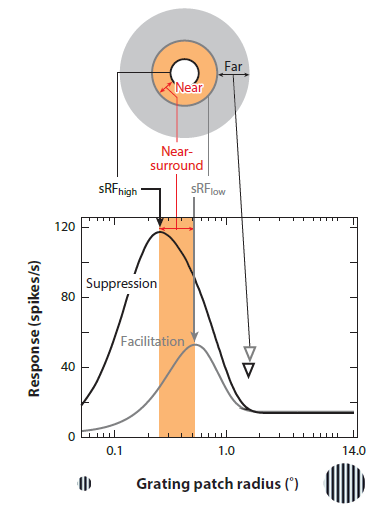
\includegraphics[scale=0.5]{2.Chapter/SMcontrast.png}
\caption{Response curves of a cell in V1 to high-contrast (black curve) and low-contrast (gray curve) as a function of the radius of displayed grating patch stimuli. The point of highest response at high-contrast is termed $sRF_{high}$ and the peak's corresponding size at low-contrast is termed $sRF_{low}$. The near surround is depicted in orange and the far surround in gray. Suppression arises in the near-surround and far-surround for high-contrast stimulation and on the other hand facilitation is evoked in the near surround and suppression in the far-surround for low-contrast gratings.
\newline \newline \tiny{Image from \cite{Angelucci2017}, adapted from experimental data tuning curves for macaque V1 in \cite{Shushruth2009}, at different contrast levels.}}
\label{SMcontrast}
\end{figure}

In this way, V1 SM has been proposed to consist on these two different components, arising from different anatomical circuits, having different tuning and spatio-temporal properties and possibly amounting to different functional perception roles \cite{Nurminen2014}. Near-SM is more strongly suppressive \cite{Shushruth2009} and more sharply tuned to orientation than far-SM. In humans, these orientation perception differences are also found similar in perceived contrast for near-surround and far-surround modulation \cite{Shushruth2013}. These different circuits can aid an efficient encoding of natural scenes \cite{Shushruth2013}. In the world, it is more statistically probable for nearby edges to belong to the same object contour if these are iso-oriented. By suppressing evoked responses for this high-occurrence contours, dependencies are minimized by tuned near-SM and the neuronal encoding is made more sparse. Moreover, decreased SM for cross-oriented lines in the near visual field can aid in object boundaries segmentation. On the other hand, for far away edges in natural scenes, statistical dependencies decrease with distance and also become less orientation dependent. Moreover, observers are more likely to perceive that two nearby edges belong to the same contour if these have the same orientation, but for far edges a wider range of orientations is possible \cite{Wertheimer1958}. Far-SM shows similar distance-dependence properties \cite{Nurminen2014}. Far-SM suppresses irrespectively of the orientation differences between edges, except when this orientation difference is very marked. This effect can thus lead to enhancement of the responses for salient distant edges, guiding saccadic eye movements and the subject's attention.

Relative to the effects mechanisms, a study has described contrast-dependent spatial integration with a difference of gaussians (DOG) model for excitatory center and inhibitory surround influences, amounting to accurate fits to contrast-dependence studies \cite{Sceniak1999}. Another study that used a receptive field model developed based on the ratio of signals from Gaussian-shaped center and surround mechanisms showed that signals from the surround modulate center responses through a divisive gain control, and that the different measurements of receptive field size according to the stimuli contrast conditions are well captured by a model in which the spatial extents of the center and surround do not change, whilst their sensitivities depend differently on stimulus contrast and stimulation history \cite{Cavanaugh2002a}. 

Regarding the circuits connections implicated with each SM component, feedforward projections from the LGN, long-range intra-V1 horizontal connections and extra-striate feedback have all been implicated. A proposal (\cite{Angelucci2002}, \cite{Angelucci2006}, \cite{Nurminen2014}) attributes these feedforward and horizontal connections to the near-surround and feedback to the far-surround (image \ref{SMconnections}).

\begin{figure}[H]
\center
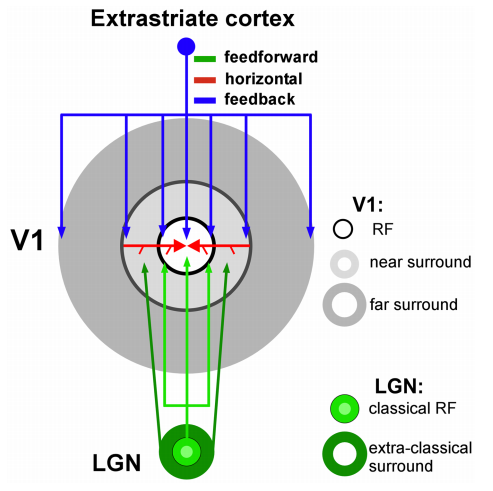
\includegraphics[scale=0.5]{2.Chapter/SMconnections.png}
\caption{The near and far components of SM and its hypothesized underlying circuits and functions. Coloured arrows indicate the different connections proposed to generate the different areas of V1 neurons - RF, near and far surround. In color code, the major functional possible roles of each connection type and surround component are presented.
\newline \newline \tiny{Image from \cite{Shushruth2013}.}}
\label{SMconnections}
\end{figure}

Feedforward contributions to SM are primarily in regards to adapting the size and tuning properties of V1 neurons (\cite{Hubel1962}, \cite{Angelucci2006}). This feedforward component to SM is fast, broadly tuned for orientation and confined to the near-surround. This component's function is suggested to be in normalizing V1 neurons' responses in regards to stimulus contrast. This is a computation found in V1 \cite{Heeger1992} that enables neurons to process wide ranges of contrast stimuli in visual scenes, despite the neurons saturation limitations \cite{Carandini2012}. There is however also evidence for a cortical contribution to untuned suppression. For example, modeling work has shown that long-range tuned suppression from horizontal connections interacting with local untuned suppression steaming from feedforward suppression effects causes SM to become tuned to the stimulus orientation presented to the cell's RF and not the cell's preferred orientation \cite{Shushruth2012}, as established from the experimental evidence for this SM property (see above, V1 SM fourth property).

Horizontal connections in V1 are most prominent in layers 2/3, come from excitatory neurons and target both excitatory and inhibitory neurons of similar orientation selectivity (\cite{Bosking1997}, \cite{Sincich2001}). This is then thought to underlie near SM tuned component. This component is proposed to be involved in the efficient encoding sparseness strategy functions of SM, aiding in object segmentation.

Finally, extrastriate feedback relays arise from excitatory neurons in layers 2/3 and 5/6 and project to both excitatory and inhibitory neurons \cite{Anderson2009}. These connections are spatially spread, and can cover the extensive far-surround modulation to V1 neurons \cite{Angelucci2002}. Feedback from different areas is fast, with connections at high conduction velocities \cite{Girard2001} and can convey information from visual field regions 5 to 25 times larger than the RF size. These properties are well suited to mediate far-SM. Moreover, recent research \cite{Nurminen2018} has shown with specific optogenetic inactivation of feedback connections, that decreasing feedback activity increases V1 neuron's RF size, decreases their responses to stimuli in the RF and increases responses to stimuli on the surround, thus decreasing surround suppression. Feedback has been implicated with attention (see subsection \ref{subsec:feedback}), as spatial attention also increases neuron's responses at attended sites \cite{McAdams2005}, modulates surrond suppression \cite{Sundberg2009} and RF size (\cite{Roberts2007}). If indeed it mediates far-SM, its properties could amount to visual salience in dissimilar stimuli at far distances, as well as the directing of saccades and attention functions. 

A working hypothesis \cite{Schwabe2006} builds on experimental proposals and biological plausability (\cite{Angelucci2017} for an evaluation of the model against available data) that SM can come from complex interactions of feedback, feedforward and horizontal connections, and implements an architecture both with increased inhibition, strong recurrency and balanced recurrent inhibition and excitation of signals (image \ref{SMmodel}). The computational model accounts for both the tuned and untuned components of SM, and works with surround stimulation activating both horizontal and feedback connections that then modulate V1's center-encoding local recurrent network, via excitatory contacts to both excitatory and two types of inhibitory neurons, one of which is tuned and the other which is untuned for orientation. This model predicted stimulus contrast and size dependences in the SM effect, later shown consistent with electrophysiology data \cite{Schwabe2010}. This result stemmed from a response asymmetry between excitation and inhibition (\cite{Somers1998}, \cite{Dragoi2000}, \cite{Schwabe2006}): For weak activation of RF center local inhibition is inactive. For strong activation of RF center, local inhibition surpasses a treshold and the center response is suppressed. 

\begin{figure}[H]
\center
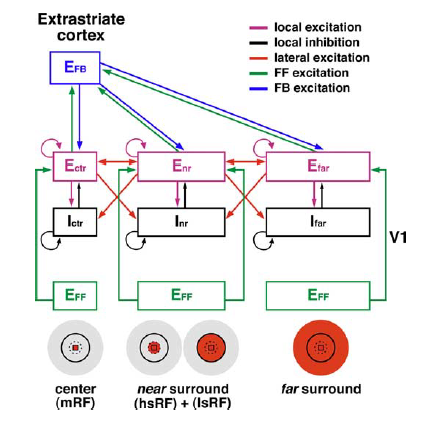
\includegraphics[scale=0.8]{2.Chapter/SMmodel.PNG}
\caption{Basic architecture of \cite{Schwabe2006} recurrent network model. Different connection types are represented as color-coded arrows. Purple and black boxes represent excitatory (E) and inhibitory (I) V1 neurons in layers 2/3 and are labeled for center, near-surround and far-surround visual field representing neurons. $E_{FF}$ green boxes represent excitatory neurons in other V1 layers that relay feedforward signals the excitatory neurons in V1 layers 2/3. The $E_{FB}$ box represent excitatory neurons in extrastriate areas that project to V1 layers 2/3 excitatory neurons. The inhibitory neurons in V1 layers 2/3 only receive direct monosynaptic input from local excitatory neurons, via local recurrent connections (purple arrows) and from horizontal connections (red arrows). 
Icons at the bottom represent the different visual field areas that are stimulated when each respective submodule is consecutively activated (from left to right) by an expanding circular stimulus.
\newline \newline \tiny{Image from \cite{Schwabe2006}.}}
\label{SMmodel}
\label{samondsnonun}
\end{figure}

This asymmetry effect does not however imply conclusive understanding of the mechanisms mediating it, as it could, for example, be implemented either with difference or divisive center-surround mechanisms, as previously presented. Notwithstanding and most fundamentally, adapted for novel data and parameter-explored for best descriptions of recent findings, these models can aind exposing the mechanisms underlying SM effects. Recurrent network models can be paramount to fully describe SM, as the non-linearity of these networks, beyond a simple feedforward ordered network, may exhibit complex behaviour that can only be explained and intuited at the appropriate non-linear paradigm.

Nevertheless, great debate is still conducted on the mechanisms that can cause SM, as well as on the circuits that mediate it. Furthermore, the functional roles of feedback are yet to be fully described, differentiated between brain areas and related to possibly separated or interacting SM effects. Finally, finding and explaining the canonical stimuli properties and components that SM effects are dependent on can also entail greater fundamental understanding of the phenomenon and its underlying networks. 

\subsection{SM non-uniformity}

As exposed in the previous section, surround modulation is currently typically studied assuming the effect's symmetry, with cat and monkey species. However, whilst the development of perceptual inference from this effect is not well understood, evidence suggests that asymmetries and different varied properties of SM are paramount for these perception processes.

In higher species, the effect has been reported complex for some neurons in the visual cortex: for these, suppression to a center line stimulus only appears when the surround stimulus is presented in given regions of the visual field - the ends (for example, \cite{Dreher1972}) or sides (for example, \cite{Born1991}) of the classical RF. This leads to width and length tuning in these cells \cite{DeAngelis1994}.

Collinear facilitation can appear: surround stimuli at the ends of the center stimulus, when coaligned with the classical RF stimulus position, can evoke an enhancement of the responses \cite{Kapadia1995}.

End-inhibition is more often present, and can lead to disambiguation of motion and disparity (\cite{Heitger1992}, \cite{Barth2000}). 

On the other hand, side-inhibition also arises from surround stimuli flanking (lateral to) the neurons' classical RF center stimuli. Along with collinear facilitation, this has been proposed to be a mechanism used for for object segmentation from a background of differently aligned stimuli \cite{Kapadia1995}. In this way, different sets of neurons show different SM effects, with individual neurons being classified as uniformly suppressed, end-inhibited, colinear-facilitated or side-inhibited by surround stimulation.

Recent advances in optogenetics and genetical identification of cells in mice have helped to unravel SM underlying circuitry (\cite{Adesnik2012}, \cite{Self2014}). 
Only more recently, SM asymmetry effects were studied in mice V1, with static line segment stimulus \cite{Samonds2017}, comparing collinear with flanking surround conditions (image \ref{samondsnonun}). This study showed that SM  for some V1 neurons in mice is indeed nonuniform in terms of collinear versus flanking surround stimulation suppression in different sets of neurons, that it is predominantly suppressive (as in higher species cases), that the nonuniform SM neurons have higher orientation selectivity and that this nonuniformity did not vary significantly with the surround's distance to the classical RF. This kind of insight in mice preparations, for which an unprecedented variety of genetic tools are available, can be leveraged to further explore SM circuits, the effect's development and its perceptual functions.

\begin{figure}[H]
\center
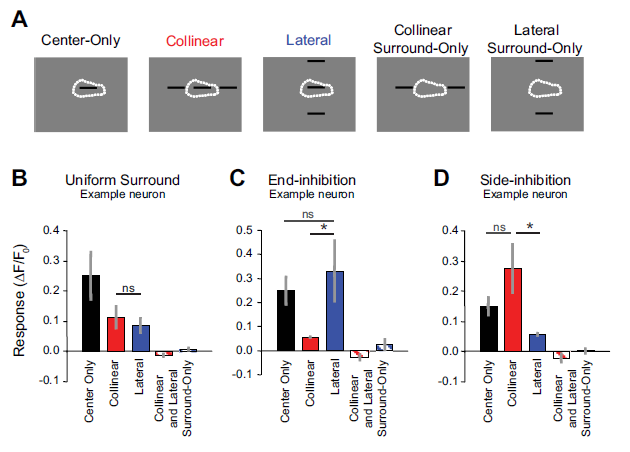
\includegraphics[scale=0.8]{2.Chapter/Samondsnonun.png}
\caption{Collinear versus lateral (flanking) stimulus conditions used in the recent nonuniformity study in mice V1.
\newline \textbf{A}: The five stimulus conditions used to test the spatial organization of the SM phenomenon.
\newline \textbf{B-D}: Behaviour of example neurons in each class of neurons: uniformly surround inhibited (B), end-inhibited (C), side-inhibited (D). In this study, colinear-facilitation was not detected, possibly due to the experimental particular settings and statistical power.
\newline \newline \tiny{Image from \cite{Samonds2017}.}}
\label{samondsnonun}
\end{figure}